% LuaLaTeX document — compile with: lualatex marine_survey_explanation.tex
\documentclass[11pt,a4paper]{article}

\usepackage{fontspec}
\setmainfont{Latin Modern Roman}
\setmonofont{Latin Modern Mono}

\usepackage{amsmath,amssymb,bm}
\usepackage{booktabs}
\usepackage{geometry}
\geometry{margin=2.5cm}
\usepackage{hyperref}
\hypersetup{colorlinks=true,linkcolor=blue!60!black,citecolor=green!50!black,urlcolor=blue!70!black}
\usepackage{enumitem}
\usepackage{xcolor}
\usepackage{tikz}
\usetikzlibrary{arrows.meta,positioning,calc,decorations.pathreplacing,patterns}

\newcommand{\D}{\Delta}
\newcommand{\order}{\mathcal{O}}
\newcommand{\bu}{\bm{u}}
\newcommand{\ee}{\mathrm{e}}
\newcommand{\ii}{\mathrm{i}}

\title{Marine Seismic Reflection Survey Simulation:\\
Towed Hydrophone Streamer with Kennett Reflectivity,\\
Ghost Operators, and Free Surface Reverberations}
\author{Research Notes}
\date{March 2026}

\begin{document}
\maketitle

\tableofcontents
\vspace{1em}

%======================================================================
\section{Motivation: synthetic shot gathers for marine surveys}
\label{sec:motivation}
%======================================================================

The CPA+Kennett pipeline computes frequency-domain reflection
coefficients $R_{PP}(\omega, p)$ for a stack of homogenised layers.
To connect this to actual marine seismic data, we need to simulate
\emph{shot gathers}---time-domain seismograms recorded at an array
of offsets from an impulsive source.

A marine towed-streamer survey introduces several effects beyond
the bare reflectivity:
\begin{enumerate}[nosep]
  \item \textbf{Water column.}  An acoustic (fluid) layer sits above
    the elastic sediments, introducing a fluid--solid interface with
    distinctive scattering coefficients.
  \item \textbf{Free surface reverberations.}  The pressure-release
    surface ($R_{\text{fs}} = -1$) traps energy in the water column,
    producing peg-leg multiples and a reverberation operator.
  \item \textbf{Source and receiver ghosts.}  A source at depth $z_s$
    below the free surface produces a delayed, polarity-reversed
    image.  Similarly for the receiver at depth $z_r$.
  \item \textbf{Offset dependence.}  The Bessel-weighted wavenumber
    summation transforms the slowness-domain reflectivity into
    offset-domain displacement.
\end{enumerate}

The module \texttt{seismic\_survey.py} implements the complete
pipeline from a YAML-configured earth model to time-domain shot
gathers, reusing the batched Kennett reflectivity from
\texttt{kennett\_layers.py} and adding the marine-specific operators
(ghosts, reverberations, Bessel summation, IFFT).

%======================================================================
\section{Survey geometry}
\label{sec:geometry}
%======================================================================

\begin{figure}[ht]
\centering
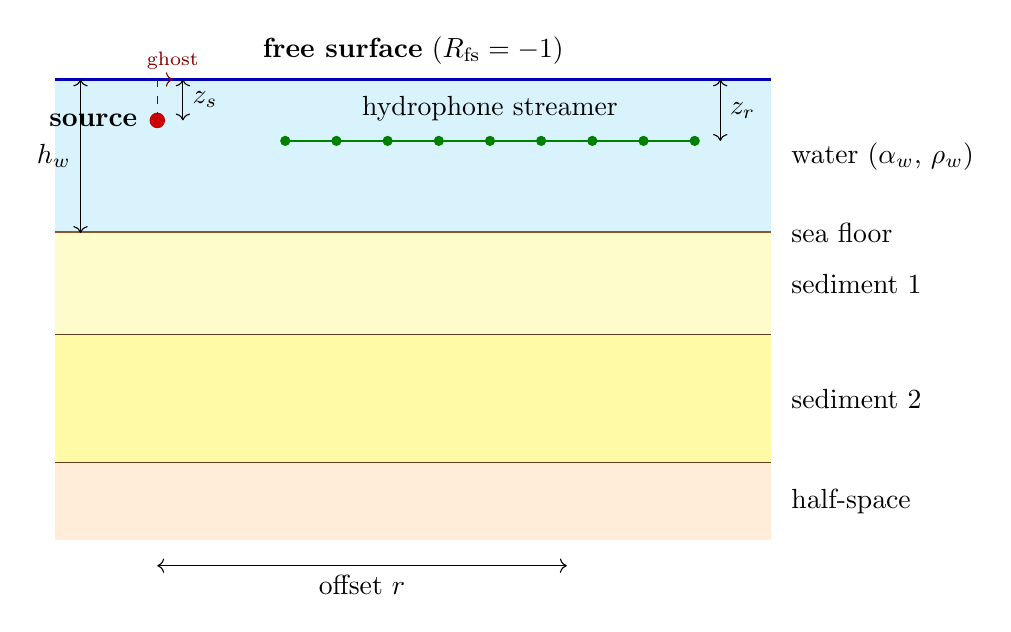
\begin{tikzpicture}[scale=0.65,
    water/.style={fill=cyan!15},
    sed/.style={fill=yellow!20},
    hs/.style={fill=orange!15}]

  % Water column
  \fill[water] (0,0) rectangle (14,-3);
  \node[right] at (14.2,-1.5) {water ($\alpha_w$, $\rho_w$)};

  % Free surface
  \draw[very thick, blue!70!black] (0,0) -- (14,0);
  \node[above] at (7,0.1) {\textbf{free surface} ($R_{\text{fs}} = -1$)};

  % Sea floor
  \draw[very thick, brown!70!black] (0,-3) -- (14,-3);
  \node[right] at (14.2,-3) {sea floor};

  % Sediment layers
  \fill[sed] (0,-3) rectangle (14,-5);
  \node[right] at (14.2,-4) {sediment 1};
  \draw[thick, brown!50!black] (0,-5) -- (14,-5);
  \fill[sed, fill=yellow!35] (0,-5) rectangle (14,-7.5);
  \node[right] at (14.2,-6.25) {sediment 2};
  \draw[thick, brown!50!black] (0,-7.5) -- (14,-7.5);
  \fill[hs] (0,-7.5) rectangle (14,-9);
  \node[right] at (14.2,-8.25) {half-space};

  % Source
  \filldraw[red!80!black] (2,-0.8) circle (4pt);
  \node[left] at (1.8,-0.8) {\textbf{source}};
  \draw[<->] (2.5,0) -- (2.5,-0.8) node[midway,right] {$z_s$};

  % Receiver array (streamer)
  \foreach \x in {4.5,5.5,...,12.5} {
    \filldraw[green!50!black] (\x,-1.2) circle (2.5pt);
  }
  \draw[thick, green!50!black] (4.5,-1.2) -- (12.5,-1.2);
  \node[above] at (8.5,-1.0) {hydrophone streamer};
  \draw[<->] (13,0) -- (13,-1.2) node[midway,right] {$z_r$};

  % Water depth
  \draw[<->] (0.5,0) -- (0.5,-3) node[midway,left] {$h_w$};

  % Offset
  \draw[<->] (2,-9.5) -- (10,-9.5) node[midway,below] {offset $r$};

  % Ghost ray paths (dashed)
  \draw[dashed, red!50!black, ->] (2,-0.8) -- (2,0) -- (2.3,0)
    node[above,font=\scriptsize] {ghost};

\end{tikzpicture}
\caption{Marine towed-streamer survey geometry.  An explosive source
at depth $z_s$ below the free surface excites P-waves that propagate
through the water column ($h_w$ deep) into the elastic sediments.
The hydrophone streamer at depth $z_r$ records pressure at offsets
$r$ from the source.  The free surface ($R_{\text{fs}} = -1$) produces
ghost reflections and water-column reverberations.}
\label{fig:geometry}
\end{figure}

The survey is parameterised by:
\begin{itemize}[nosep]
  \item Source depth $z_s$ (typically 5--10~m) and receiver depth
    $z_r$ (typically 6--12~m).
  \item Receiver type: \texttt{hydrophone} (pressure sensor,
    standard for marine) or \texttt{geophone} (velocity sensor,
    ocean-bottom).
  \item Water column: depth $h_w$, velocity $\alpha_w$ (typically
    1500~m/s), density $\rho_w$ (typically 1025~kg/m$^3$).
  \item Receiver offsets $r_1, \ldots, r_{n_r}$ (m).
\end{itemize}

The earth model below the water is a stack of isotropic elastic
layers $(\alpha_i, \beta_i, \rho_i, h_i)$ terminated by a
half-space, represented as a \texttt{LayerStack} with a
\texttt{FluidLayer} on top.

%======================================================================
\section{The fluid layer and fluid--solid interface}
\label{sec:fluid}
%======================================================================

\subsection{The FluidLayer dataclass}

A new \texttt{FluidLayer} class represents an acoustic layer with
$\beta = 0$ (no shear support).  This is distinct from
\texttt{IsotropicLayer} which requires $\beta > 0$.  The
\texttt{LayerStack} type is relaxed to
\texttt{Sequence[FluidLayer\,|\,IsotropicLayer]}.

\subsection{Fluid--solid scattering coefficients}

At the ocean bottom, the upper layer is acoustic ($\beta_1 = 0$,
$\eta^S_1 = 0$) and the lower layer is elastic.  The modified
P-SV scattering coefficients simplify from the general solid--solid
case~\cite{kennett1983}.

The intermediate variables $a$, $b$, $c$, $d$ are the same as
for solid--solid, but with $\mu_1 = 0$:
\begin{equation}\label{eq:abcd}
  d = 2\rho_2 \beta_2^2, \quad
  a = \D\rho - p^2 d, \quad
  b = \rho_2 - p^2 d, \quad
  c = \rho_1 + p^2 d.
\end{equation}
The coupling terms simplify because $\eta^S_1 = 0$:
\begin{equation}\label{eq:EFGH}
  E = b\,\eta_1 + c\,\eta_2, \quad
  F = b, \quad
  G = a - d\,\eta_1\,\eta^S_2, \quad
  H = -d\,\eta_2.
\end{equation}
Compare with the solid--solid case where $F = b\,\eta^S_1 + c\,\eta^S_2$
and $H = a - d\,\eta_2\,\eta^S_1$.

The determinant is:
\begin{equation}
  \D = EF + GH\,p^2.
\end{equation}

After normalising by $\D$ and computing the six scattering amplitudes
$T_1, \ldots, T_6$, the $2\times 2$ matrices have
acoustic--elastic sparsity:
\begin{equation}\label{eq:Rd_sparse}
  R^d = \begin{pmatrix} R^d_{PP} & 0 \\ 0 & 0 \end{pmatrix}, \quad
  T^d = \begin{pmatrix} T^d_{PP} & 0 \\ T^d_{SP} & 0 \end{pmatrix}, \quad
  T^u = \begin{pmatrix} T^u_{PP} & T^u_{PS} \\ 0 & 0 \end{pmatrix}, \quad
  R^u = \begin{pmatrix} R^u_{PP} & R^u_{PS} \\ R^u_{SP} & R^u_{SS} \end{pmatrix}.
\end{equation}

The acoustic layer cannot support downgoing S-waves (column~1 of
$T^d$ is zero) or upgoing S-waves (row~1 of $T^u$ is zero).  The
elastic layer's upgoing reflection $R^u$ is full $2 \times 2$
because P-to-S conversion occurs at the ocean bottom.

At normal incidence ($p \to 0$), $R^d_{PP}$ reduces to the
acoustic impedance formula:
\begin{equation}\label{eq:impedance}
  R^d_{PP} \to \frac{Z_2 - Z_1}{Z_2 + Z_1}, \qquad
  Z_i = \rho_i\,\alpha_i.
\end{equation}

%======================================================================
\section{Kennett reflectivity}
\label{sec:kennett}
%======================================================================

\subsection{Recursive algorithm}

The Kennett upward-sweep recursion~\cite{kennett1983} builds
the cumulative downgoing reflection matrix $\overline{R}^D$
by sweeping from the half-space upward:
\begin{equation}\label{eq:kennett}
  \overline{R}^D = R^d + T^u\;E^2\,\overline{R}^D_{\text{below}}\;
    \bigl(\bm{I} - R^u\;E^2\,\overline{R}^D_{\text{below}}\bigr)^{-1}\;T^d,
\end{equation}
where $E^2$ is the two-way phase delay through the layer below
the current interface:
\begin{equation}
  E^2 = \text{diag}\bigl(\ee^{2\ii\omega\eta h},\;
    \ee^{2\ii\omega\eta^S h}\bigr).
\end{equation}

At each interface, the recursion dispatches to either
\texttt{psv\_fluid\_solid()} or \texttt{psv\_solid\_solid()}
depending on the layer types.

\subsection{Batched computation}
\label{sec:batched}

For the survey simulation, the reflectivity must be evaluated
at every $(p, \omega)$ pair in the slowness--frequency grid.
The function \texttt{kennett\_reflectivity\_batch()} vectorises
this using 4D arrays of shape $(n_p, n_\omega, 2, 2)$.

The scattering coefficients at each interface are precomputed
for all $n_p$ slowness values (they are frequency-independent):
\begin{equation}
  R^d_{\text{all}},\;R^u_{\text{all}},\;T^d_{\text{all}},\;T^u_{\text{all}}
  \;\in\;\mathbb{C}^{n_{\text{iface}} \times n_p \times 2 \times 2}.
\end{equation}

The phase factors broadcast over both dimensions:
\begin{equation}
  E_\alpha[i, j_p, j_\omega]
  = \exp\bigl(\ii\,\eta_i(p_{j_p})\;\omega_{j_\omega}\;h_i\bigr).
\end{equation}

The Kennett recursion then uses \texttt{np.matmul} broadcasting
for all $2 \times 2$ operations, with a custom analytical
$2 \times 2$ batch inverse that supports arbitrary leading
dimensions via \texttt{[...]} indexing.

The output is the PP component:
$\overline{R}^D_{PP}(p, \omega) \in \mathbb{C}^{n_p \times n_\omega}$.

%======================================================================
\section{Free surface reverberations}
\label{sec:freesurface}
%======================================================================

The ocean is a reverberant waveguide bounded by:
\begin{itemize}[nosep]
  \item \textbf{Top:} pressure-release free surface
    ($R_{\text{fs}} = -1$).
  \item \textbf{Bottom:} sub-ocean cumulative reflectivity
    $\overline{R}^D_{PP}$.
\end{itemize}

Applying the Kennett addition rule to the water column gives the
total reflectivity including all water-column multiples:
\begin{equation}\label{eq:reverb}
  \boxed{R_{\text{total}}
  = \frac{E_w^2\;\overline{R}^D_{PP}}
         {1 + E_w^2\;\overline{R}^D_{PP}},}
\end{equation}
where $E_w^2 = \exp(2\ii\omega\,\eta_w\,h_w)$ is the two-way
P-wave phase through the water column, and the denominator
encodes the free surface reflection $R_{\text{fs}} = -1$.

Expanding as a geometric series:
\begin{equation}\label{eq:geom}
  R_{\text{total}} = E_w^2\,\overline{R}^D
    - E_w^4\,(\overline{R}^D)^2
    + E_w^6\,(\overline{R}^D)^3
    - \cdots
\end{equation}
Each term adds another round trip through the ocean ($E_w^2$)
and another sub-ocean reflection ($\overline{R}^D$), with
alternating sign from $R_{\text{fs}} = -1$.  The first term is
the primary reflection; subsequent terms are peg-leg multiples.

For weak sub-ocean reflectivity ($|\overline{R}^D| \ll 1$),
the total reflectivity is dominated by the primary:
$R_{\text{total}} \approx E_w^2\,\overline{R}^D$.

%======================================================================
\section{Ghost operators}
\label{sec:ghosts}
%======================================================================

\subsection{Source ghost}

An explosive source at depth $z_s$ below the free surface
generates a direct downgoing wave and a delayed, polarity-reversed
upgoing wave reflected from the surface.  In the frequency--slowness
domain:
\begin{equation}\label{eq:source_ghost}
  G_s(\omega, p) = 1 - \exp(2\ii\omega\,q_w\,z_s),
\end{equation}
where $q_w = \sqrt{1/\alpha_w^2 - p^2}$ is the vertical slowness
in water.  At zero depth ($z_s = 0$), $G_s = 0$---the source and
its ghost cancel exactly.

The source ghost has notch frequencies where the ghost destructively
interferes with the direct arrival.  At normal incidence ($p = 0$):
\begin{equation}
  f_{\text{notch}} = \frac{n\,\alpha_w}{2\,z_s}, \quad n = 1, 2, 3, \ldots
\end{equation}
For $z_s = 5$~m and $\alpha_w = 1500$~m/s, the first notch is at
$f = 150$~Hz.

\subsection{Receiver ghost}

The receiver ghost depends on the sensor type:
\begin{equation}\label{eq:receiver_ghost}
  G_r(\omega, p) = \begin{cases}
    1 + \exp(2\ii\omega\,q_w\,z_r) & \text{hydrophone (pressure)}, \\
    1 - \exp(2\ii\omega\,q_w\,z_r) & \text{geophone (velocity)}.
  \end{cases}
\end{equation}

For a \textbf{hydrophone}, the free surface doubles the pressure
(constructive interference at $z_r = 0$: $G_r = 2$).
For a \textbf{geophone}, the velocity reverses at the free surface
(destructive at $z_r = 0$: $G_r = 0$).

The ghost operators are applied as multiplicative factors in
the $(p, \omega)$ domain:
\begin{equation}
  R_{\text{observed}} = R_{\text{total}} \cdot G_s \cdot G_r.
\end{equation}

%======================================================================
\section{Bessel summation: slowness to offset}
\label{sec:bessel}
%======================================================================

The discrete wavenumber method~\cite{bouchon1981} transforms the
slowness-domain reflectivity $R(p, \omega)$ to offset-domain
spectral displacement:
\begin{equation}\label{eq:bessel}
  U(r, \omega)
  = \D p \sum_{j=1}^{n_p}
    R(p_j, \omega)\;J_0(\omega\,p_j\,r)\;p_j\;\omega,
\end{equation}
where $J_0$ is the zeroth-order Bessel function of the first kind,
$\D p = p_{\max} / n_p$ is the slowness spacing, and $r$ is the
source--receiver offset.

\subsection{Hann taper}

To suppress Gibbs ringing from the abrupt truncation at
$p_{\max}$, a Hann (cosine) taper is applied to the slowness
integration:
\begin{equation}
  w(p) = \frac{1}{2}\Bigl(1 + \cos\frac{\pi\,p}{p_{\max}}\Bigr).
\end{equation}
This smoothly reduces the integrand to zero at $p_{\max}$, trading
slightly reduced resolution for near-critical phases against
clean suppression of truncation artefacts.

\subsection{GPU acceleration}

The Bessel summation is the computational bottleneck
($n_p \times n_r \times n_\omega$ operations).  The GPU version
(\texttt{bessel\_summation\_gpu}) processes slowness samples in
chunks of 256, transferring the weighted reflectivity and Bessel
function values to GPU for an \texttt{einsum} accumulation:
\begin{equation}
  U_{\text{re}}[r, \omega] = \sum_j J_0[r, j, \omega]\;W_{\text{re}}[j, \omega],
\end{equation}
with separate real/imaginary passes in float32 (the Bessel arguments
and amplitudes are $\order(1)$, so single precision is adequate).

%======================================================================
\section{Source spectrum}
\label{sec:source}
%======================================================================

The default source is a Ricker wavelet with peak frequency $f_p$:
\begin{equation}\label{eq:ricker}
  S(\omega) = \Bigl(\frac{\omega}{\omega_p}\Bigr)^2
    \exp\!\Bigl[-\Bigl(\frac{\omega}{\omega_p}\Bigr)^2\Bigr],
    \qquad \omega_p = 2\pi f_p.
\end{equation}
This is a zero-phase, band-limited wavelet with:
\begin{itemize}[nosep]
  \item $S(0) = 0$ (no DC component),
  \item Peak at $\omega = \omega_p$ where $S = \ee^{-1} \approx 0.368$,
  \item Rapid Gaussian roll-off above the peak.
\end{itemize}

The source spectrum is applied after the Bessel summation, as a
multiplicative factor in the frequency domain:
$U(r, \omega) \leftarrow U(r, \omega) \cdot S(\omega)$.

%======================================================================
\section{IFFT and damping compensation}
\label{sec:ifft}
%======================================================================

Following Bouchon~\cite{bouchon1981}, the reflectivity is computed at
complex frequencies $\omega + \ii\gamma$ to suppress temporal aliasing
from the discrete slowness integration.  The damping factor is:
\begin{equation}
  \gamma = \frac{\pi}{T},
\end{equation}
where $T$ is the record length.

The time-domain seismogram is recovered by:
\begin{enumerate}[nosep]
  \item Building a Hermitian-symmetric spectrum from $U(r, \omega)$:
    \begin{equation}
      \tilde{U}[k] = \begin{cases}
        0 & k = 0, \\
        U[r, k] & k = 1, \ldots, n_w{-}1, \\
        0 & k = n_w, \\
        \overline{U[r, 2n_w{-}k]} & k = n_w{+}1, \ldots, 2n_w{-}1.
      \end{cases}
    \end{equation}
  \item Computing $u(r, t) = \text{Re}\bigl[\text{FFT}(\tilde{U})\bigr]$.
  \item Compensating the exponential growth:
    $u(r, t) \leftarrow u(r, t) \cdot \ee^{-\gamma t}$.
\end{enumerate}

The final time axis is $t_k = k\,T / (2 n_w)$ for
$k = 0, \ldots, 2n_w - 1$.

%======================================================================
\section{Complete pipeline}
\label{sec:pipeline}
%======================================================================

The function \texttt{compute\_shot\_gather()} chains all steps:

\begin{center}
\renewcommand{\arraystretch}{1.3}
\begin{tabular}{rll}
\toprule
\textbf{Step} & \textbf{Operation} & \textbf{Output shape} \\
\midrule
1 & Build frequency grid $\omega + \ii\gamma$ & $(n_\omega,)$ \\
2 & Build slowness grid $p_j = j\,\D p$ & $(n_p,)$ \\
3 & Batched Kennett reflectivity (sub-ocean) & $(n_p, n_\omega)$ \\
4 & Water-column phase $E_w^2$ & $(n_p, n_\omega)$ \\
5 & Free surface reverberations (optional) & $(n_p, n_\omega)$ \\
6 & Source ghost $\times$ receiver ghost & $(n_p, n_\omega)$ \\
7 & Bessel summation & $(n_r, n_\omega)$ \\
8 & Source spectrum & $(n_r, n_\omega)$ \\
9 & IFFT + damping compensation & $(n_r, n_t)$ \\
\bottomrule
\end{tabular}
\end{center}

\noindent
The sub-ocean stack (layers below water) is extracted and passed
to \texttt{kennett\_reflectivity\_batch()}.  The water-column
effects (ghosts, reverberations) are applied separately in the
$(p, \omega)$ domain.  This separation allows the sub-ocean
reflectivity to be reused with different survey configurations.

%======================================================================
\section{Connection to the three-level architecture}
\label{sec:architecture}
%======================================================================

The marine survey simulator sits atop the CPA+Kennett pipeline,
adding the observation layer:

\begin{center}
\renewcommand{\arraystretch}{1.3}
\begin{tabular}{lp{5cm}p{5cm}}
\toprule
\textbf{Level} & \textbf{Module} & \textbf{Role} \\
\midrule
Inner
  & \texttt{effective\_contrasts.py}
  & Single-cube T-matrix \\
Middle
  & \texttt{cpa\_iteration.py}
  & CPA self-consistent homogenisation \\
Outer (1D)
  & \texttt{kennett\_layers.py}
  & Kennett layer stacking + batched reflectivity \\
Observation
  & \texttt{seismic\_survey.py}
  & Marine survey effects + synthetic gathers \\
\bottomrule
\end{tabular}
\end{center}

The survey module can work with either:
\begin{itemize}[nosep]
  \item \textbf{Direct earth model:} layers specified in the
    YAML configuration as $(\alpha, \beta, \rho, h)$.
  \item \textbf{CPA-homogenised model:} layers built from
    \texttt{cpa\_stack\_from\_phases()} with a water column
    prepended by \texttt{build\_survey\_stack()}.
\end{itemize}

%======================================================================
\section{Implementation details}
\label{sec:implementation}
%======================================================================

\subsection{Module structure}

The module \texttt{seismic\_survey.py} provides:

\begin{center}
\renewcommand{\arraystretch}{1.2}
\begin{tabular}{lp{8.5cm}}
\toprule
\textbf{Class / Function} & \textbf{Purpose} \\
\midrule
\texttt{SurveyConfig} &
  Dataclass: source/receiver depths, offsets, water properties,
  receiver type (\texttt{hydrophone} or \texttt{geophone}). \\
\texttt{GatherConfig} &
  Dataclass: frequency band, record length, slowness grid,
  source wavelet, free surface flag. \\
\texttt{ShotGatherResult} &
  Dataclass: time axis, offsets, gather array $(n_r, n_t)$,
  raw reflectivity $(n_p, n_\omega)$, layer stack. \\
\midrule
\texttt{source\_ghost} &
  $G_s(\omega, p)$: explosive source ghost. \\
\texttt{receiver\_ghost} &
  $G_r(\omega, p)$: hydrophone or geophone ghost. \\
\texttt{free\_surface\_reverberations} &
  $R = E^2 \overline{R}^D / (1 + E^2 \overline{R}^D)$. \\
\texttt{ricker\_source\_spectrum} &
  $S(\omega) = (\omega/\omega_p)^2 \exp[-(\omega/\omega_p)^2]$. \\
\texttt{bessel\_summation} &
  CPU Bessel-weighted wavenumber summation. \\
\texttt{bessel\_summation\_gpu} &
  GPU-accelerated version (PyTorch + chunked einsum). \\
\texttt{build\_survey\_stack} &
  Water \texttt{FluidLayer} + sediments + half-space $\to$
  \texttt{LayerStack}. \\
\texttt{compute\_shot\_gather} &
  Main entry point: full pipeline $\to$ \texttt{ShotGatherResult}. \\
\texttt{load\_survey\_config} &
  Parse YAML $\to$ (\texttt{LayerStack}, \texttt{SurveyConfig},
  \texttt{GatherConfig}). \\
\bottomrule
\end{tabular}
\end{center}

\noindent
The \texttt{kennett\_layers.py} additions:

\begin{center}
\renewcommand{\arraystretch}{1.2}
\begin{tabular}{lp{8.5cm}}
\toprule
\textbf{Class / Function} & \textbf{Purpose} \\
\midrule
\texttt{FluidLayer} &
  Acoustic layer: $\alpha$, $\rho$, $h$; $\beta = 0$ enforced. \\
\texttt{psv\_fluid\_solid} &
  Modified P-SV coefficients at fluid--solid interface. \\
\texttt{kennett\_reflectivity\_batch} &
  Vectorised Kennett over $(n_p, n_\omega)$ with 4D arrays. \\
\bottomrule
\end{tabular}
\end{center}

\subsection{Units}

All quantities use SI units (m, s, kg, Pa):
\begin{itemize}[nosep]
  \item Velocities in m/s (not km/s as in the PhD reference code).
  \item Slowness in s/m (not s/km).
  \item Offsets in m (not km).
  \item Frequencies in rad/s.
\end{itemize}

\subsection{YAML configuration}

\begin{verbatim}
# configs/example_survey.yml
survey:
  source_depth: 5.0          # m
  receiver_depth: 8.0        # m
  receiver_type: hydrophone
  water_depth: 70.0          # m (Bass Strait)
  water_alpha: 1500.0        # m/s
  water_rho: 1025.0          # kg/m^3
  offsets:
    min: 100.0               # m
    max: 3000.0
    spacing: 12.5

gather:
  f_min: 5.0                 # Hz
  f_max: 80.0
  T: 4.0                     # s record length
  nw: 4096
  np_slow: 8192
  free_surface: true
  source:
    type: ricker
    f_peak: 30.0             # Hz

earth_model:
  layers:
    - {alpha: 1600, beta: 300, rho: 1800, thickness: 50}
    - {alpha: 2200, beta: 800, rho: 2100, thickness: 200}
    - {alpha: 3500, beta: 1800, rho: 2400, thickness: 300}
    - {alpha: 5000, beta: 3000, rho: 2700, thickness: inf}
\end{verbatim}

\subsection{Typical workflow}

\begin{verbatim}
from cubic_scattering import (
    SurveyConfig, GatherConfig, IsotropicLayer,
    build_survey_stack, compute_shot_gather,
)
import numpy as np

# 1. Survey geometry
survey = SurveyConfig(
    source_depth=5.0, receiver_depth=8.0,
    receiver_type="hydrophone",
    offsets=np.arange(100, 3001, 12.5),
    water_depth=70.0,
)

# 2. Earth model
sediments = [
    IsotropicLayer(1600, 300, 1800, 50),
    IsotropicLayer(2200, 800, 2100, 200),
    IsotropicLayer(3500, 1800, 2400, 300),
]
half_space = IsotropicLayer(5000, 3000, 2700, np.inf)
stack = build_survey_stack(survey, sediments, half_space)

# 3. Compute shot gather
gc = GatherConfig(f_peak=30.0, free_surface=True)
result = compute_shot_gather(stack, survey, gc)

# 4. Access time-domain gather
print(result.gather.shape)  # (nr, nt)
\end{verbatim}

\subsection{Parameter selection guide}

\begin{center}
\renewcommand{\arraystretch}{1.3}
\begin{tabular}{lp{9cm}}
\toprule
\textbf{Parameter} & \textbf{Guidance} \\
\midrule
$n_w$ (frequencies) &
  Controls frequency resolution $\D f = 1/T$.
  4096 gives $\D f = 0.25$~Hz at $T = 4$~s. \\
$n_p$ (slowness samples) &
  Controls spatial aliasing.  8192 with auto $p_{\max}$ is
  adequate for most models. \\
$p_{\max}$ &
  Auto-computed as $1.2 / \alpha_{\min}$.  Increase for
  wide-angle reflections near the critical angle. \\
$\gamma$ (damping) &
  Default $\pi / T$.  Larger values suppress artefacts
  more aggressively but reduce resolution. \\
$T$ (record length) &
  Must exceed the two-way travel time to the deepest
  reflector of interest.  4~s for shallow water, 8+~s for deep. \\
\bottomrule
\end{tabular}
\end{center}

%======================================================================
\section{Validation}
\label{sec:validation}
%======================================================================

The module is validated by 31 tests across 12 test classes.
The existing 46 Kennett tests continue to pass (regression).

\subsection{Ghost operators}

\begin{itemize}[nosep]
  \item Zero source depth gives $G_s = 0$ (exact cancellation).
  \item Zero receiver depth gives $G_r = 2$ for hydrophone
    (pressure doubling) and $G_r = 0$ for geophone.
  \item Source ghost notch at $f = \alpha_w / (2z_s)$ verified
    to tolerance $10^{-6}$.
  \item Hydrophone $+$ geophone $= 2$ at all frequencies
    (complementary polarity).
\end{itemize}

\subsection{Free surface reverberations}

\begin{itemize}[nosep]
  \item $\overline{R}^D = 0$ gives $R_{\text{total}} = 0$.
  \item $|\overline{R}^D| = 1$ gives bounded $R_{\text{total}}$
    (no blow-up).
  \item For small $\overline{R}^D$, first-order expansion
    matches to 2\%.
\end{itemize}

\subsection{Fluid--solid interface}

\begin{itemize}[nosep]
  \item $R^d$ has only $[0,0]$ nonzero.
  \item $T^d$ column~1 is zero.
  \item $T^u$ row~1 is zero.
  \item Exact match against PhD \texttt{ocean\_bottom\_interface()}
    at 5 slowness values (tolerance $10^{-14}$).
  \item Normal-incidence $R^d_{PP}$ matches impedance formula
    \eqref{eq:impedance} to 1\%.
\end{itemize}

\subsection{Batched Kennett}

\begin{itemize}[nosep]
  \item Batched result matches scalar \texttt{kennett\_layers()} at
    3 selected $(p, \omega)$ pairs to tolerance $10^{-12}$.
  \item Fluid--solid stack produces nonzero reflectivity.
\end{itemize}

\subsection{End-to-end gather}

\begin{itemize}[nosep]
  \item Output shapes are correct: $(n_r, 2n_w)$.
  \item Gather has nonzero energy (reflections are present).
  \item YAML configuration loads correctly, producing the right
    layer count (water + sediments + half-space).
\end{itemize}

%======================================================================
\section{Future extensions}
\label{sec:future}
%======================================================================

\begin{enumerate}
  \item \textbf{CPA-homogenised survey.}  Build the sub-ocean stack
    from \texttt{cpa\_stack\_from\_phases()}, producing a
    frequency-dependent earth model.

  \item \textbf{Multiple receiver types.}  Ocean-bottom node
    simulation with both hydrophones and geophones at the sea floor
    ($z_r = h_w$).

  \item \textbf{Attenuation (Q).}  Pass $Q_\alpha$, $Q_\beta$ from
    the YAML config through to the layer stack for intrinsic
    absorption.

  \item \textbf{AVO extraction.}  Extract amplitude-versus-offset
    curves from the synthetic gathers for comparison with
    Zoeppritz equations.

  \item \textbf{Source directivity.}  Replace the isotropic
    explosive source with an airgun array directivity pattern.

  \item \textbf{Full waveform inversion.}  Use the synthetic
    gathers as forward-modelled data for FWI benchmarking.
\end{enumerate}

%======================================================================
\section{References}
%======================================================================

\begin{thebibliography}{99}

\bibitem{kennett1983}
B.L.N.\ Kennett,
\emph{Seismic Wave Propagation in Stratified Media},
Cambridge University Press (1983).

\bibitem{bouchon1981}
M.\ Bouchon,
``A simple method to calculate Green's functions for elastic
layered media,''
\emph{Bull.\ Seismol.\ Soc.\ Am.}\ \textbf{71}(4), 959--971 (1981).

\bibitem{slabdoc}
``3D Slab Foldy--Lax Multiple Scattering Solver,''
companion document,
\texttt{docs/slab\_scattering\_explanation.pdf} (2026).

\bibitem{cubeeshelby}
``Self-Consistent T-Matrix for Cubic Scatterers,''
companion document,
\texttt{docs/cube\_eshelby\_explanation.pdf} (2026).

\bibitem{aki1980}
K.\ Aki, P.G.\ Richards,
\emph{Quantitative Seismology: Theory and Methods},
W.H.\ Freeman (1980).

\end{thebibliography}

\end{document}
